%% 
%% Copyright 2007, 2008, 2009 Elsevier Ltd
%% 
%% This file is part of the 'Elsarticle Bundle'.
%% ---------------------------------------------
%% 
%% It may be distributed under the conditions of the LaTeX Project Public
%% License, either version 1.2 of this license or (at your option) any
%% later version.  The latest version of this license is in
%%    http://www.latex-project.org/lppl.txt
%% and version 1.2 or later is part of all distributions of LaTeX
%% version 1999/12/01 or later.
%% 
%% The list of all files belonging to the 'Elsarticle Bundle' is
%% given in the file `manifest.t\textbf{xt}'.
%% 

%% Template article for Elsevier's document class `elsarticle'
%% with numbered style bibliographic references
%% SP 2008/03/01

\documentclass[preprint,review,11pt]{elsarticle}

%% Use the option review to obtain double line spacing
%%\documentclass[authoryear,preprint,review,12pt]{elsarticle}

%% Use the options 1p,twocolumn; 3p; 3p,twocolumn; 5p; or 5p,twocolumn
%% for a journal layout:
%% \documentclass[final,1p,times]{elsarticle}
%% \documentclass[final,1p,times,twocolumn]{elsarticle}
%% \documentclass[final,3p,times]{elsarticle}
%% \documentclass[final,3p,times,twocolumn]{elsarticle}
%% \documentclass[final,5p,times]{elsarticle}
%% \documentclass[final,5p,times,twocolumn]{elsarticle}

%% For including figures, graphicx.sty has been loaded in
%% elsarticle.cls. If you prefer to use the old commands
%% please give \usepackage{epsfig}

%% The amssymb package provides various useful mathematical symbols
\usepackage{amssymb}
%% The amsthm package provides extended theorem environments
%% \usepackage{amsthm}

%% The lineno packages adds line numbers. Start line numbering with
%% \begin{linenumbers}, end it with \end{linenumbers}. Or switch it on
%% for the whole article with \linenumbers.
%% \usepackage{lineno}

\usepackage{fullpage}
\usepackage{amsfonts}
\usepackage{graphicx}
\usepackage{amsmath}
\usepackage{indentfirst}
\usepackage[version=3]{mhchem} % Formula subscripts using \ce{}
\usepackage[T1]{fontenc}       % Use modern font encodings

\usepackage{float}
\usepackage{chemfig}
\usepackage{longtable}
\usepackage{array}
\usepackage{cellspace}
\usepackage{palatino}
%\usepackage{breqn}
\usepackage{amssymb}
\usepackage{verbatim}
\usepackage[colorlinks=true,citecolor=blue,linkcolor=blue]{hyperref}
\usepackage{siunitx}
\usepackage{xr}
\usepackage{adjustbox}
\usepackage{lscape}

\usepackage{setspace}

%%% Old arguments
%\usepackage{graphicx}
%% uncomment according to your operating system:
%% ------------------------------------------------
%\usepackage[latin1]{inputenc}    %% european characters can be used (Windows, old Linux)
%%\usepackage[utf8]{inputenc}     %% european characters can be used (Linux)
%%\usepackage[applemac]{inputenc} %% european characters can be used (Mac OS)
%% ------------------------------------------------
%\usepackage{authblk}
%\usepackage[superscript]{cite}
%\usepackage[document]{ragged2e}
%\usepackage[T1]{fontenc}   %% get hyphenation and accented letters right
%\usepackage{mathptmx}      %% use fitting times fonts also in formulas
%% do not change these lines:
%\pagestyle{empty}                %% no page numbers!
%\usepackage[left=35mm, right=35mm, top=15mm, bottom=20mm, noheadfoot]{geometry}
%%% please don't change geometry settings!
%
%\usepackage{fullpage}
%\usepackage{amsfonts}
%\usepackage{graphicx}
%\usepackage{float}
%\usepackage{amsmath}
%\usepackage{chemfig}
%\usepackage{indentfirst}
%\usepackage{longtable}
%\usepackage{array}
%\usepackage{cellspace}
%\usepackage{palatino}
%%\usepackage{breqn}
%\usepackage{amssymb}
%\usepackage{verbatim}
%\usepackage[colorlinks=true,citecolor=blue,linkcolor=blue]{hyperref}
%\usepackage{siunitx}
%\usepackage{xr}

%% italicized boldface for math (e.g. vectors)
%\newcommand{\bfv}[1]{{\mbox{\boldmath{$#1$}}}}
%% non-italicized boldface for math (e.g. matrices)
%\newcommand{\bfm}[1]{{\bf #1}}          
%
%%\newcommand{\bfm}[1]{{\mbox{\boldmath{$#1$}}}}
%%\newcommand{\bfm}[1]{{\bf #1}}
%\newcommand{\expect}[1]{\left \langle #1 \right \rangle} % <.> for denoting expectations over realizations of an experiment or thermal averages
%
%\newcommand{\var}[1]{{\mathrm var}{(#1)}}
%\newcommand{\x}{\bfv{x}}
%\newcommand{\y}{\bfv{y}}
%\newcommand{\f}{\bfv{f}}
%
%\newcommand{\hatf}{\hat{f}}
%
%\newcommand{\bTheta}{\bfm{\Theta}}
%\newcommand{\btheta}{\bfm{\theta}}
%\newcommand{\bhatf}{\bfm{\hat{f}}}
%\newcommand{\Cov}[1] {\mathrm{cov}\left( #1 \right)}
%\newcommand{\T}{\mathrm{T}}                                % T used in matrix transpose
%
%\newcommand\blfootnote[1]{%
%	\begingroup
%	\renewcommand\thefootnote{}\footnote{#1}%
%	\addtocounter{footnote}{-1}%
%	\endgroup
%}

\newenvironment{myequation}{%
	\addtocounter{equation}{-1}
	\refstepcounter{defcounter}
	\renewcommand\theequation{SI.\thedefcounter}
	\begin{equation*}}
{\end{equation*}}

\renewcommand{\thefigure}{SI.\arabic{figure}}

\renewcommand{\thepage}{SI.\arabic{page}}

\renewcommand{\thesection}{SI.\Roman{section}}

\renewcommand{\thetable}{SI.\Roman{table}}

\makeatletter
\newcommand*{\addFileDependency}[1]{% argument=file name and extension
	\typeout{(#1)}
	\@addtofilelist{#1}
	\IfFileExists{#1}{}{\typeout{No file #1.}}
}
\makeatother

\newcommand*{\myexternaldocument}[1]{%
	\externaldocument{#1}%
	\addFileDependency{#1.tex}%
	\addFileDependency{#1.aux}%
}

\myexternaldocument{IFPSC_10_manuscript}

% The figures are in a figures/ subdirectory.
\graphicspath{{figures/}}

\journal{Fluid Phase Equilibria}

\begin{document}
	
	\begin{frontmatter}
		
		%% Title, authors and addresses
		
		%% use the tnoteref command within \title for footnotes;
		%% use the tnotetext command for theassociated footnote;
		%% use the fnref command within \author or \address for footnotes;
		%% use the fntext command for theassociated footnote;
		%% use the corref command within \author for corresponding author footnotes;
		%% use the cortext command for theassociated footnote;
		%% use the ead command for the email address,
		%% and the form \ead[url] for the home page:
		%% \title{Title\tnoteref{label1}}
		%% \tnotetext[label1]{}
		%% \author{Name\corref{cor1}\fnref{label2}}
		%% \ead{email address}
		%% \ead[url]{home page}
		%% \fntext[label2]{}
		%% \cortext[cor1]{}
		%% \address{Address\fnref{label3}}
		%% \fntext[label3]{}
		
		\title{Supporting Information: Mie 16-6 force field predicts viscosity with faster-than-exponential pressure dependence for 2,2,4-trimethylhexane}
		
		%% use optional labels to link authors explicitly to addresses:
		%% \author[label1,label2]{}
		%% \address[label1]{}
		%% \address[label2]{}
		
		\author{Richard A. Messerly}
		\ead{richard.messerly@nist.gov}
		\address{Thermodynamics Research Center, National Institute of Standards and Technology, Boulder, Colorado, 80305}
		
		\author{Michelle C. Anderson}
		\ead{michelle.anderson@nist.gov}
		\address{Thermodynamics Research Center, National Institute of Standards and Technology, Boulder, Colorado, 80305}
		
		\author{S. Mostafa Razavi}
		\address{Department of Chemical and Biomolecular Engineering, The University of Akron, Akron, Ohio, 44325-3906}
        \ead{sr87@zips.uakron.edu}
		
		\author{J. Richard Elliott}
		\address{Department of Chemical and Biomolecular Engineering, The University of Akron, Akron, Ohio, 44325-3906}
		\ead{elliot1@uakron.edu}
				
	\end{frontmatter}	
		
	\section{Input files} \label{SI:Gromacs input files}
	
	We provide example input files for simulating 2,2,4-trimethylhexane at 293 K with the Potoff force field in GROMACS (see attached .gro, .top, and .mdp files). Additionally, all files necessary to generate the results from this study can be found at \newline www.github.com/ramess101/IFPSC\_10.
	
    \clearpage
	\newpage
	
	\section{MCMC from scoring function} \label{SI:MCMC from scoring function}
	
	Markov Chain Monte Carlo (MCMC) requires an expression for the likelihood function $(L)$ and, in particular, the log (or natural log) of the likelihood function ($\ln(L)$). For example, by assuming a uniform prior in the model parameters and a symmetric proposal distribution, the Metropolis-Hastings acceptance criterion for an MCMC move only depends on $L$ such that
	\begin{equation}
	\alpha = \frac{L(D|\theta_{\rm new})}{L(D|\theta_{\rm old})}
	\end{equation}
	where $D$ are the data, $\theta$ are the model parameters, and $\alpha$ is the probability of accepting a proposed or ``new'' parameter set ($\theta_{\rm new}$) given a previous or ``old'' parameter set ($\theta_{\rm old}$). For computational reasons, it is common to perform MCMC using the log-likelihood such that 
	\begin{equation} \label{eq:log-alpha}
	\ln(\alpha) = \ln(L(D|\theta_{\rm new})) - \ln(L(D|\theta_{\rm old}))
	\end{equation}
	By contrast, Mick et al. optimize the Potoff CH and C parameters using a scoring function $(S)$ that weights the deviations for several different properties and their derivatives. This section describes how we translate the scoring function into a log-likelihood function, to then implement in MCMC.
	
	\subsection{Derivation}
		
	Standard least-squares minimization is mathematically equivalent to maximizing the likelihood function when assuming the errors follow a normal distribution. This can be readily verified from the following expression
	\begin{multline} \label{eq:likelihood}
	L(D|\theta) = \prod_i \frac{1}{\sqrt{2 \pi \sigma^{2}}} \exp\left[\frac{-1}{2\sigma^2}(y(\theta)-D_i)^2\right] = \frac{1}{\sqrt{2 \pi^n \sigma^{2n}}} \exp\left[\frac{-1}{2\sigma^2}\left(\sum_i(y(\theta)-D_i)^2\right)\right] \\ = \frac{1}{\sqrt{2 \pi^n \sigma^{2n}}} \exp\left(\frac{-SSE(\theta)}{2\sigma^2}\right)
	\end{multline}
	where $n$ is the number of data points, $\sigma$ is the standard deviation (which is assumed to be equal for all data points), $y(\theta)$ is the model estimate, and $\sum_i(y(\theta)-D_i)^2$ is the sum-squared-error $(SSE)$. The log-likelihood can then be expressed as    
	\begin{equation} \label{eq:log-likelihood}
%	\ln(L(D|\theta)) = \ln\left(\frac{1}{\sqrt{2 \pi^n \sigma^{2n}}}\right) - \frac{SSE(\theta)}{2\sigma^2}
    \ln(L(D|\theta)) = \frac{-1}{2}\ln\left(2 \pi^n \sigma^{2n}\right) - \frac{SSE(\theta)}{2\sigma^2}
	\end{equation}  
	Substitution of Equation \ref{eq:log-likelihood} into Equation \ref{eq:log-alpha} yields the MCMC acceptance probability
	\begin{equation}
	\ln(\alpha) = \frac{SSE(\theta_{\rm old}) - SSE(\theta_{\rm new})}{2\sigma^2}
	\end{equation}
	which only depends on $SSE$ and $\sigma$. Note that the order of ``new'' and ``old'' changes due to the negative sign in Equation \ref{eq:log-likelihood}. Also, note the cancellation of the first term on the right-hand-side of Equation \ref{eq:log-likelihood}, as it does not depend on $\theta$.
	
	%Clearly, minimizing the sum-squared-error is mathematically equivalent to maximizing the likelihood or log-likelihood when assuming the errors follow a normal distribution.
	
	To this point, we have assumed that the standard deviation is constant with respect to the data. Relaxing this assumption, the likelihood is expressed as
	\begin{multline} \label{eq:weighted-likelihood}
	L(D|\theta) = \prod_i \frac{1}{\sqrt{2 \pi \sigma_i^{2}}} \exp\left[\frac{-1}{2\sigma_i^2}(y(\theta)-D_i)^2\right] = C \exp\left[\sum_i\frac{-1}{2\sigma_i^2}(y(\theta)-D_i)^2\right] \\ = C \exp\left[\sum_i-w_i(y(\theta)-D_i)^2\right] = C \exp\left(-WSSE(\theta)\right)
	\end{multline}
	where $\sigma_i$ varies for $D_i$, $C$ is a normalization constant equal to $\prod_i (2 \pi \sigma_i^2)^{-1/2}$, and $WSSE$ is the weighted-sum-squared-error with weights $(w_i)$ equal to $\sigma_i^{-2}$. Thus, minimizing $WSSE$ with $w_i = \sigma_i^{-2}$ is also equivalent to the maximum likelihood approach assuming normally distributed errors, but where the standard deviations are not constant with respect to the data. The log-likelihood can then be expressed as    
	\begin{equation} \label{eq:weighted-log-likelihood}
	\ln(L(D|\theta)) = \ln(C) - WSSE(\theta)
	\end{equation}
	and substitution into Equation \ref{eq:log-alpha} yields the MCMC acceptance probability
	\begin{equation}
	\ln(\alpha) = WSSE(\theta_{\rm old}) - WSSE(\theta_{\rm new})
	\end{equation}
	which only depends on $WSSE$.
	
	
	Potoff's scoring function $(S)$ is not simply the sum-squared-error or even the weighted-sum-squared-error. $S$ is expressed in terms of the absolute percent deviation and each property is assigned a different weight that is not necessarily the inverse variance ($\sigma_i^{-2}$). Therefore, minimizing $S$ is not equivalent to maximizing the likelihood of a normal distribution for neither constant nor varying $\sigma$. However, we can still apply the maximum likelihood criterion for Potoff's scoring function such that
%	\begin{multline} \label{eq:scoring-likelihood}
%	L(D|\theta) = \prod_i C_i \exp\left[w_i|y(\theta)-D_i|\right] = C \exp\left[\sum_i w_i|y(\theta)-D_i|\right] \\ = C \exp\left(-S(\theta)\right)
%	\end{multline}
	\begin{equation} \label{eq:scoring-likelihood}
	L(D|\theta) = \prod_i C_i \exp\left(w_i\left|\frac{y(\theta)-D_i}{D_i}\right|\right) = C \exp\left(\sum_i w_i\left|\frac{y(\theta)-D_i}{D_i}\right|\right) = C \exp\left(-S(\theta)\right)
	\end{equation}
	where $C_i$ and $C$ are normalization constants, and $w_i$ are the weights assigned by Potoff (e.g., 0.6135 for saturated liquid density). Note that although Equation \ref{eq:scoring-likelihood} utilizes an absolute percent deviation, rather than a weighted-sum-squared-error, the final expression is still analogous to Equation \ref{eq:weighted-likelihood}. Therefore, the log-likelihood for Potoff's scoring function is
	\begin{equation}
	\ln(L(D|\theta)) = \ln(C) -S(\theta)
	\end{equation}
	and substitution into Equation \ref{eq:log-alpha} yields the MCMC acceptance probability
	\begin{equation} \label{eq:log-score}
	\ln(\alpha) = S(\theta_{\rm old}) - S(\theta_{\rm new})
	\end{equation}
	which only depends on Potoff's scoring function, $S$.
	
	%%%%%%%%%%%%%%%%%%%%%%%%%%%%%%%%% Rough draft
%	
%	Mick et al. optimized the Potoff CH and C parameters using a scoring function $(S)$ that weights the deviations for several different properties and their derivatives. MCMC requires an expression for the likelihood function $(L)$ and, in particular, the log (or natural log) of the likelihood function ($\ln(L)$). This section describes how we translate the scoring function into a log-likelihood function.
%	
%	Standard least squares minimization is mathematically equivalent to maximizing the likelihood function of a normal distribution. This can be readily verified from the following expression
%	\begin{multline} \label{eq:likelihood}
%	L(D|\theta) = \prod_i \frac{1}{\sqrt{2 \pi \sigma^{2}}} \exp\left[\frac{-1}{2\sigma^2}(y(\theta)-D_i)^2\right] = \frac{1}{\sqrt{2 \pi^n \sigma^{2n}}} \exp\left[\frac{-1}{2\sigma^2}\left(\sum_i(y(\theta)-D_i)^2\right)\right] \\ = \frac{1}{\sqrt{2 \pi^n \sigma^{2n}}} \exp\left(\frac{-SSE(\theta)}{2\sigma^2}\right)
%	\end{multline}
%	where $D$ are the data, $\theta$ are the model parameters, $n$ is the number of data points, $\sigma$ is the standard deviation (which is assumed to be equal for all data points), $y(\theta)$ is the model estimate, and $\sum_i(y(\theta)-D_i)^2$ is the sum-squared-error $(SSE)$. The log-likelihood can then be expressed as    
%	\begin{equation} \label{eq:log-likelihood}
%	\ln(L(D|\theta)) = \ln\left(\frac{1}{\sqrt{2 \pi^n \sigma^{2n}}}\right) - \frac{SSE(\theta)}{2\sigma^2}
%	\end{equation}  
%	Clearly, minimizing the sum-squared-error is mathematically equivalent to maximizing the likelihood or log-likelihood when assuming the errors follow a normal distribution. 
%	
%	In MCMC, assuming a uniform prior, the probability of accepting a proposed or ``new'' parameter set ($\theta_{\rm new}$) given a previous or ``old'' parameter set ($\theta_{\rm old}$) is
%	\begin{equation}
%	\alpha = \frac{L(D|\theta_{\rm new})}{L(D|\theta_{\rm old})}
%	\end{equation}
%	where $\alpha$ is the acceptance probability. For computational reasons, it is common to perform MCMC using the log-likelihood such that 
%	\begin{equation} \label{eq:log-alpha}
%	\ln(\alpha) = \ln(L(D|\theta_{\rm new})) - \ln(L(D|\theta_{\rm old}))
%	\end{equation}
%	Note that the term in Equation \ref{eq:log-likelihood} that does not depend on $\theta$ cancels when computing $\ln(\alpha)$. Substitution of Equation \ref{eq:log-likelihood} into Equation \ref{eq:log-alpha} yields
%	\begin{equation}
%	\ln(\alpha) = \frac{SSE(\theta_{\rm old}) - SSE(\theta_{\rm new})}{2\sigma^2}
%	\end{equation}
%	note that the order of ``new'' and ``old'' changes due to the negative sign in Equation \ref{eq:log-likelihood}. 
%	
%	To this point, we have assumed that the standard deviation is constant with respect to the data. Relaxing this assumption, the likelihood is expressed as
%	\begin{multline} \label{eq:weighted-likelihood}
%	L(D|\theta) = \prod_i \frac{1}{\sqrt{2 \pi \sigma_i^{2}}} \exp\left[\frac{-1}{2\sigma_i^2}(y(\theta)-D_i)^2\right] = C \exp\left[\sum_i\frac{-1}{2\sigma_i^2}(y(\theta)-D_i)^2\right] \\ = C \exp\left[\sum_i-w_i(y(\theta)-D_i)^2\right] = C \exp\left(-WSSE(\theta)\right)
%	\end{multline}
%	where $\sigma_i$ varies for $D_i$, $C$ is a normalization constant equal to $\prod_i (2 \pi \sigma_i^2)^{-1}$, and $WSSE$ is the weighted-sum-squared-error with weights $(w_i)$ equal to $\sigma_i^{-2}$. The log-likelihood can then be expressed as    
%	\begin{equation} \label{eq:weighted-log-likelihood}
%	\ln(L(D|\theta)) = \ln(C) - WSSE(\theta)
%	\end{equation}
%	and substitution into Equation \ref{eq:log-alpha} yields the MCMC acceptance probability for the weighted-sum-squared-error
%	\begin{equation}
%	\ln(\alpha) = WSSE(\theta_{\rm old}) - WSSE(\theta_{\rm new})
%	\end{equation}
%	
%	Potoff's scoring function $(S)$ is not simply the sum-squared-error or even the weighted-sum-squared-error. $S$ is expressed in terms of the absolute percent deviation and different properties are assigned different weights that are not necessarily the inverse variance ($\sigma_i^{-2}$). Therefore, minimizing $S$ is not equivalent to maximizing the likelihood of a normal distribution for neither constant nor varying $\sigma$. However, we can still apply the maximum likelihood criterion for Potoff's scoring function such that
%	%	\begin{multline} \label{eq:scoring-likelihood}
%	%	L(D|\theta) = \prod_i C_i \exp\left[w_i|y(\theta)-D_i|\right] = C \exp\left[\sum_i w_i|y(\theta)-D_i|\right] \\ = C \exp\left(-S(\theta)\right)
%	%	\end{multline}
%	\begin{equation} \label{eq:scoring-likelihood}
%	L(D|\theta) = \prod_i C_i \exp\left(w_i\left|\frac{y(\theta)-D_i}{D_i}\right|\right) = C \exp\left(\sum_i w_i\left|\frac{y(\theta)-D_i}{D_i}\right|\right) = C \exp\left(-S(\theta)\right)
%	\end{equation}
%	where $C_i$ and $C$ are normalization constants, and $w_i$ are the weights assigned by Potoff (e.g., 0.6135 for saturated liquid density, $\rho_{\rm liq}$). Note that although Equation \ref{eq:scoring-likelihood} utilizes an absolute percent deviation, rather than a weighted-sum-squared-error, the final expression is still analogous to Equation \ref{eq:weighted-likelihood}. Therefore, the log-likelihood for Potoff's scoring function is
%	\begin{equation}
%	\ln(L(D|\theta)) = \ln(C) -S(\theta)
%	\end{equation}
%	and substitution into Equation \ref{eq:log-alpha} yields the MCMC acceptance probability for Potoff's scoring function
%	\begin{equation} \label{eq:log-score}
%	\ln(\alpha) = S(\theta_{\rm old}) - S(\theta_{\rm new})
%	\end{equation}
%	
	%%%%%%%%%%%%%%%%%%%%%%%%%%%%%%%%%%%%%%%%%%%
	
	% for the i$^{\rm th}$ data point. Note that $w_i$ incorporates both the coefficients Potoff assigns (e.g., 0.6135 for $\rho_{\rm liq}$) as well as the inverse data value $(1/D_i)$. 
%	
%Substituting $S$ for $WSSE$ in Equations \ref{eq:weighted-likelihood}.
%	
%    The reason we group the $(2\sigma^2)^{-1}$ term into the scoring function is because $S$ already contains weighting terms. A standard weighted least squares approach is to assign weights based on the inverse variance ($\sigma^2$). For example,  different weights to the , which are essentially 
%	and, therefore, the MCMC acceptance probability is simply
%	\begin{equation} \label{eq:log-score}
%	\ln(\alpha) = S(\theta_{\rm old}) - S(\theta_{\rm new})
%	\end{equation}
%	
%	\begin{multline} \label{eq:likelihood}
%	L(D|\theta) = \prod_i C_i \exp\left[w_i(y(\theta)-D_i)\right] = C \exp\left[\sum_i w_i(y(\theta)-D_i)\right] \\ = C \exp\left(-S(\theta)\right)
%	\end{multline}
%	where $C_i$ and $C$ are normalization constants, and $w_i$ is the weight for the i$^{\rm th}$ data point. Note that $w_i$ incorporates both the coefficients Potoff assigns in the scoring function  The log-likelihood can then be expressed as    
%	\begin{equation}
%	\ln(L(D|\theta)) = \ln(C) - S(\theta)
%	\end{equation}
%	and, therefore, the MCMC acceptance probability is simply
%	\begin{equation} \label{eq:log-score}
%	\ln(\alpha) = S(\theta_{\rm old}) - S(\theta_{\rm new})
%	\end{equation}
%	
%	However, we can still apply the maximum likelihood criterion by substituting $S$ for $SSE/(2\sigma^2)$ in Equation \ref{eq:log-likelihood}
%	\begin{equation}
%	\ln(L(D|\theta)) \propto -S(\theta)
%	\end{equation}
%	The reason we group the $(2\sigma^2)^{-1}$ term into the scoring function is because $S$ already contains weighting terms. A standard weighted least squares approach is to assign weights based on the inverse variance ($\sigma^2$). For example,  different weights to the , which are essentially 
%	and, therefore, the MCMC acceptance probability is simply
%	\begin{equation} \label{eq:log-score}
%	\ln(\alpha) = S(\theta_{\rm old}) - S(\theta_{\rm new})
%	\end{equation}
%	
%	Potoff's scoring function $(S)$ is not simply the sum-squared-error. $S$ is expressed in terms of the percent deviation and different properties are assigned different weights. Therefore, minimizing $S$ is not equivalent to maximizing the likelihood of a normal distribution. However, we can still apply the maximum likelihood criterion by substituting $S$ for $SSE/(2\sigma^2)$ in Equation \ref{eq:log-likelihood}. The reason we group the $(2\sigma^2)^{-1}$ term into the scoring function is because $S$ already contains weighting terms. A standard weighted least squares approach is to assign weights based on the inverse variance ($\sigma^2$). So, effectively, we are
%	\begin{multline} \label{eq:likelihood}
%	L(D|\theta) = \prod_i C_i \exp\left[w_i(y(\theta)-D_i)\right] = C \exp\left[\sum_i w_i(y(\theta)-D_i)\right] \\ = C \exp\left(-S(\theta)\right)
%	\end{multline}
%	where $C_i$ and $C$ are normalization constants, and $w_i$ is the weight for the i$^{\rm th}$ data point. The log-likelihood can then be expressed as    
%	\begin{equation}
%	\ln(L(D|\theta)) = \ln(C) - S(\theta)
%	\end{equation}
%	and, therefore, the MCMC acceptance probability is simply
%	\begin{equation} \label{eq:log-score}
%	\ln(\alpha) = S(\theta_{\rm old}) - S(\theta_{\rm new})
%	\end{equation}
	
	%%% Original text
	
%	Mick et al. optimized the Potoff CH and C parameters using a scoring function $(S)$ that weights the deviations for several different properties and their derivatives. MCMC requires an expression for the likelihood function $(L)$ and, in particular, the log of the likelihood function (log$_{10}(L)$). This section describes how we translate the scoring function into a log-likelihood function.
%	
%	Standard least squares minimization is mathematically equivalent to maximizing the likelihood function of a normal distribution. This can be readily verified from the following expression
%	\begin{multline} \label{eq:likelihood}
%	L(D|\theta) = \prod_i \frac{1}{\sqrt{2 \pi \sigma^{2}}} \exp\left[\frac{-1}{2\sigma^2}(y(\theta)-D_i)^2\right] = \frac{1}{\sqrt{2 \pi^n \sigma^{2n}}} \exp\left[\frac{-1}{2\sigma^2}\left(\sum_i(y(\theta)-D_i)^2\right)\right] \\ = \frac{1}{\sqrt{2 \pi^n \sigma^{2n}}} \exp\left(\frac{-SSE(\theta)}{2\sigma^2}\right)
%	\end{multline}
%	where $D$ are the data, $\theta$ are the model parameters, $n$ is the number of data points, $\sigma$ is the standard deviation, $y(\theta)$ is the model estimate, and $\sum(y(\theta)-D_i)^2$ is the sum-squared-error $(SSE)$. The log-likelihood can then be expressed as    
%	\begin{equation} \label{eq:log-likelihood}
%	\log_{10}(L(D|\theta)) = \log_{10}(\frac{1}{\sqrt{2 \pi^n \sigma^{2n}}}) - \frac{SSE(\theta)}{2\sigma^2}
%	\end{equation}  
%	Clearly, minimizing the sum-squared-error is mathematically equivalent to maximizing the likelihood or log-likelihood when assuming the errors follow a normal distribution. 
%	
%%	\begin{equation} \label{eq:log-likelihood}
%%	\log_{10}(L(D|\theta)) \propto -\sum(y(\theta)-D_i)^2 \propto -SSE(\theta)
%%	\end{equation} 
%	
%%	\begin{equation} \label{eq:likelihood}
%%	L(D|\theta) = \frac{1}{\sqrt{2 \pi^n \sigma^{2n}}}\exp\left[\frac{-1}{2\sigma^2}\left(\sum_i(y(\theta)-D_i)^2\right)\right]
%%	\end{equation}
%	
%	
%%	 by expressing the likelihood function for the product of normal distributions with standard deviation $\sigma$ and the average $\mu$ can be seen easily by expressing
%	
%% of the proposed or ``new'' parameter set $\theta_{\rm old}$ is the previous or ``old'' parameter set, and  is the proposed or ``new'' parameter set.
%
%    In MCMC, assuming a uniform prior, the probability of accepting a proposed or ``new'' parameter set ($\theta_{\rm new}$) given a previous or ``old'' parameter set ($\theta_{\rm old}$) is
%    \begin{equation}
%    \alpha = \frac{L(D|\theta_{\rm new})}{L(D|\theta_{\rm old})}
%    \end{equation}
%    where $\alpha$ is the acceptance probability. For computational reasons, it is common to perform MCMC using the log-likelihood such that 
%    \begin{equation} \label{eq:log-alpha}
%    \log_{10}(\alpha) = \log_{10}(L(D|\theta_{\rm new})) - \log_{10}(L(D|\theta_{\rm old}))
%    \end{equation}
%    Note that all terms in Equation \ref{eq:likelihood} that do not depend on $\theta$ cancel when computing log$_{10}(\alpha)$. Assuming a normal distribution or, equivalently, minimizing $SSE$ is achieved in MCMC by substituting Equation \ref{eq:log-likelihood} into Equation \ref{eq:log-alpha} which yields
%    \begin{equation}
%    \log_{10}(\alpha) = \sum(y(\theta_{\rm old})-D_i)^2 - \sum(y(\theta_{\rm new})-D_i)^2 = SSE(\theta_{\rm old}) - SSE(\theta_{\rm new})
%    \end{equation}
%    note that the order of ``new'' and ``old'' changes due to the negative sign in Equation \ref{eq:log-likelihood}. 
%
%    Because Potoff's scoring function $(S)$ is not simply the sum-squared-error, minimizing $S$ is not equivalent to maximizing the likelihood of a normal distribution. However, we can still apply the maximum likelihood criterion by substituting $S$ for $SSE$ in Equation \ref{eq:log-likelihood}
%    \begin{equation}
%    \log_{10}(L(D|\theta)) \propto -S(\theta)
%    \end{equation}
%    and, therefore, the MCMC acceptance probability is simply
%    \begin{equation} \label{eq:log-score}
%    \log_{10}(\alpha) = S(\theta_{\rm old}) - S(\theta_{\rm new})
%    \end{equation}
    
%     Again, because the terms that do not depend on $\theta$ cancel when taking the difference of logarithms, the acceptance probability is just
%	\begin{equation}
%	\log_{10}(alpha) = S_{\rm old} - S_{\rm new}
%	\end{equation}  
%	\begin{equation}
%	log_{10}(L(D|\theta)) \propto -S(\theta)
%	\end{equation}
%	
%	\begin{equation}
%	log_{10}(L(D|\theta)) \propto -SSE(\theta)
%	\end{equation}

    \subsection{Implementation}

    With Equation \ref{eq:log-score}, all that remains to perform MCMC is a way to compute $S$ for any $\theta$. This is achieved by smoothing/interpolating the raw scoring function values (utilizing SciPy's RectBivariateSpline function in the interpolation sub-package\footnote{https://docs.scipy.org/doc/scipy/reference/generated/scipy.interpolate.RectBivariateSpline.html}) over the two-dimensional grids of $\epsilon_{\rm CH}$-$\sigma_{\rm CH}$ and $\epsilon_{\rm C}$-$\sigma_{\rm C}$. The values of $S$ were obtained through private communication with Potoff's group. Only the scoring function values from the ``long'' CH and C parameters are utilized in this study. Using the ``generalized'' or ``short'' scoring function values would result in a different MCMC sampling of $\epsilon$ and $\sigma$.
	
	The optimal ``long'' CH parameter is on the boundary of the grid tested by Mick et al. Therefore, we do not have any simulation scoring function values for $\epsilon_{\rm CH} < 14$ K. A similar problem is faced for $\epsilon_{\rm C} < 0.8$ K and $\sigma_{\rm C} > 0.63$ nm but, fortunately, these regions are rarely sampled by the MCMC algorithm. To overcome the challenge of extrapolating outside of the domain where $S(\theta)$ is available, we fit $\ln(S(\theta))$ to a multi-variate normal distribution. This approach works well for the CH parameters because the CH scoring function has a fairly normal shape. While the assumption of normality is worse for $S$ over the $\epsilon_{\rm C}$-$\sigma_{\rm C}$ parameter space, this does not significantly affect our results because of the infrequent sampling of this extrapolation region.   



%    In MCMC, the probability of accepting a new parameter set only depends on the log-likelihood (assuming a uniform prior), which for Equation \ref{eq:likelihood} 
%    \begin{equation}
%    log_{10}(L(D|\theta)) \propto -\sum(y(\theta)-D_i)^2 \propto -SSE(\theta)
%    \end{equation}
%	
%    In MCMC, the probability of accepting a new parameter set is equal to the difference between log$_{10}(L(D|\theta_{\rm new}))$ and log$_{10}(L(D|\theta_{\rm old}))$ (assuming a uniform prior). All terms in Equation \ref{eq:likelihood} that do not depend on $\theta$ cancel. Therefore, the acceptance probability $(\alpha)$ is equal to
%    \begin{equation}
%    \alpha = \sum(y(\theta_{\rm old})-D_i)^2 - \sum(y(\theta_{\rm new})-D_i)^2 = SSE_{\rm old} - SSE_{\rm new}
%    \end{equation}
%    \begin{multline}
%    \alpha = log_{10}(L(D|\theta_{\rm new})) - log_{10}(L(D|\theta_{\rm old})) = \sum(y(\theta_{\rm old})-D_i)^2 - \sum(y(\theta_{\rm new})-D_i)^2 = SSE_{\rm old} - SSE_{\rm new}
%    \end{multline}
%    note that the order of ``new'' and ``old'' changes due to the negative sign in Equation \ref{eq:likelihood}.
%    
 
    
%      After taking the logarithm of Equation \ref{eq:likelihood}, and subtracting log$_{10}(L(D|\theta_{\rm new}))$ and log$_{10}(L(D|\theta_{\rm old}))$ log$_{10}((L)$ and omi By removing all terms that 
%	
%	 Similarly, minimization of Potoff's scoring function $(S)$ is mathematically equivalent to maximizing log$_{10}(L(S))$.  the log  Translating the scoring function into a Bayesian context is actually quite simple. 
%	
%	Translating the scoring function into a Bayesian context is achieved by modeling the $\epsilon$-$\sigma$ CH and C uncertainties with a multivariate normal distribution, where the covariance matrix was obtained by assuming that the ``generalized'' CH and C parameter set should not be distinguishable (at the 95~\% confidence level) from the ``long'' parameter set.
%	
%	We apply the common assumption of transferability between UA sites, which implies that the parameter correlation between different UA sites, e.g., between $\sigma_{\rm CH_3}$ and $\sigma_{\rm CH}$, is assumed to be negligible. In other words, we only account for the parameter correlation between $\epsilon_{ii}$-$\sigma_{ii}$ sets of the same UA site. The reason for this assumption is the reduced complexity of performing four independent two-dimensional MCMC runs compared to one eight-dimensional MCMC run.
%	
    \clearpage
    \newpage

	\section{MCMC validation} \label{SI:MCMC_analysis}
	
	This section validates the combined bootstrap re-sampling and MCMC approach. Specifically, we compare the uncertainties (depicted as histograms) obtained in two different manners. First, as in the main text, a single replicate simulation is performed for each MCMC-nb parameter set and the results are pooled together for bootstrap re-sampling ($N_{\rm reps} = 1$, $N_{\rm MCMC} = 40$). Second, 40 replicate simulations are performed for 30 sets of MCMC-nb parameters, bootstrap re-sampling is performed independently for each set of 40 replicates, and the overall uncertainty is obtained by combining the 30 bootstrapped distributions ($N_{\rm reps} = 40$, $N_{\rm MCMC} = 30$). Due to the large amount of simulations required for this comparison, we perform this analysis on a simpler system, namely, ethane at 137 K and saturated liquid density using the Potoff force field. 
	
	Figure \ref{fig:MCMC_validation} demonstrates that the uncertainties are nearly indistinguishable for the two methods. This provides empirical evidence that performing a single simulation with each MCMC parameter set provides the same uncertainty as performing numerous simulations with each MCMC parameter set. Also of interest is that the numerical uncertainties ($N_{\rm reps} = 40$, $N_{\rm MCMC} = 1$) are much smaller than the overall uncertainties, suggesting that parameter uncertainty plays a larger role for ethane than for the challenge compound.
	
	\begin{figure}[htb!]
		\centering
		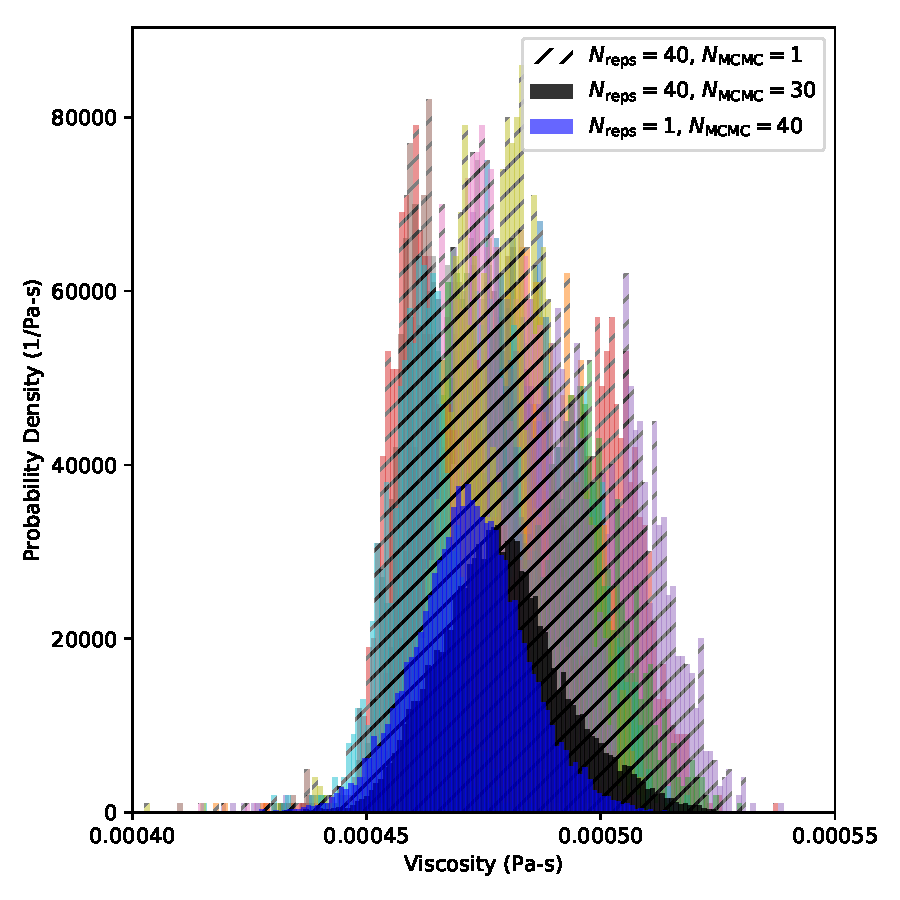
\includegraphics[width=3.2in]{MCMC_validation.pdf}
		\caption{Validation of combined bootstrap re-sampling and MCMC approach utilized in study. Note that the uncertainties are almost indistinguishable between $(N_{\rm reps} = 1$, $N_{\rm MCMC} = 40)$ and $(N_{\rm reps} = 40$, $N_{\rm MCMC} = 30)$.}
		\label{fig:MCMC_validation}
	\end{figure}
	
    \clearpage
	\newpage
	
    \section{Torsion parameter uncertainty} \label{SI:MCMC torsions}
	
%	Sensitivity 
%	Nieto did 15 and 40
%	-40 has very strange torsional barriers
%	+80 did not seem justified for a single data point
%	
%	 
%	
%	As only a single viscosity data point is available for  In order to determine how much th
%	
%	
%	While Nieto-Draghi et al. propose that the internal and terminal torsions be increased by 15~\% and 40~\%, respectively,  
	
	
	In this section, we develop the skewed normal distribution for $A_{\rm s}$, where the respective lower and upper 95~\% confidence intervals correspond to -15~\% and +40~\% of the maximum torsional barrier. The viscosity values obtained with Potoff are considerably higher than those obtained with AUA4. Therefore, it is feasible, especially at higher pressures, that the optimal value of $A_{\rm s}$ is negative, i.e., the viscosity may be too high and, thus, decreasing the torsional barriers might improve the viscosity estimates. For this reason, unlike Nieto-Draghi et al., we also consider $A_{\rm s} < 0$.
	
	To determine the appropriate scaling of the torsional barriers, Figure \ref{fig:sensitivity_torsions} presents a sensitivity analysis of $\eta$ with respect to $A_{\rm s}$. $A_{\rm s}$ is expressed as a percentage of the maximum for the non-shifted torsional potential. The viscosities in Figure \ref{fig:sensitivity_torsions} for 2,2,4-trimethylhexane are computed at 293 K and atmospheric pressure with 200 molecules and the Potoff force field. Also depicted is the only available experimental viscosity value at the same temperature and saturation pressure. 	 
	
	\begin{figure}[htb!]
		\centering
				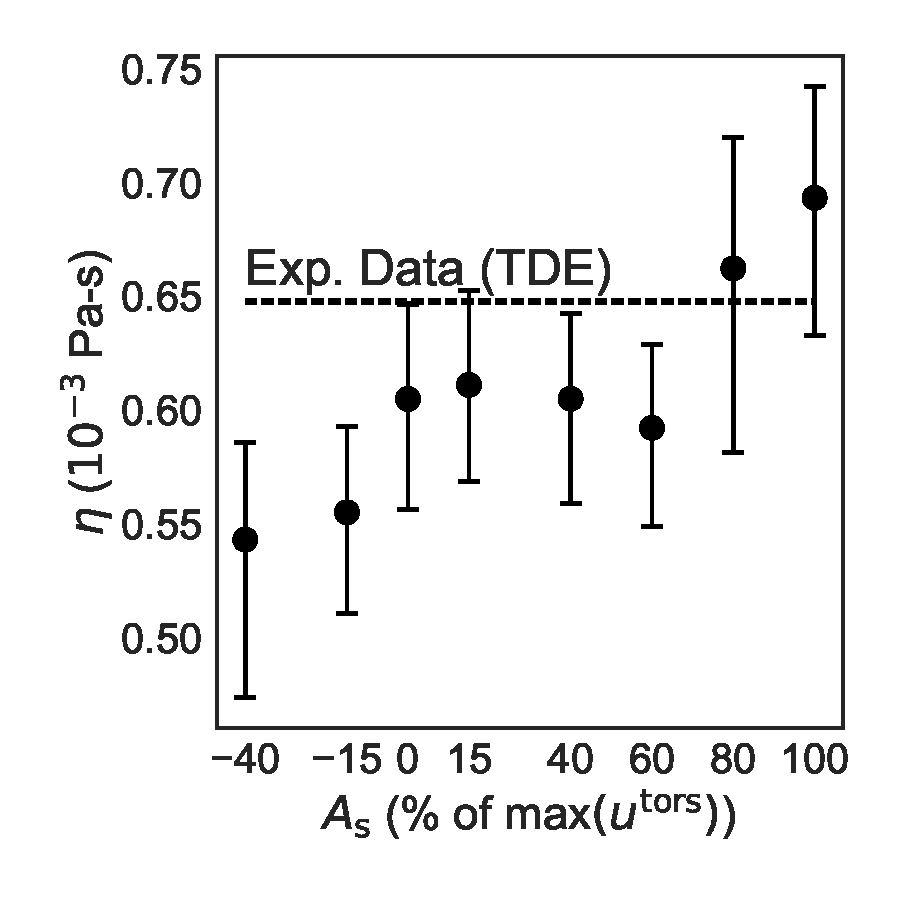
\includegraphics[width=3.2in]{sensitivity_torsions.pdf}
		\caption{Sensitivity analysis of viscosity to torsional barrier heights. Simulations are performed at 293 K and atmospheric pressure. Experimental data are depicted as a dashed line. Uncertainties are expressed at 95~\% confidence level, where the experimental uncertainty is approximately the line-width.}
		\label{fig:sensitivity_torsions}
	\end{figure}
	
%	As the Mie 16-6 potential predicts $\eta$ more accurately than the Lennard-Jones 12-6 potentials, 
	
	Figure \ref{fig:sensitivity_torsions} demonstrates that quantitative agreement with the experimental viscosity point necessitates an $A_{\rm s}$ value that is 80~\% the maximum torsional barrier. Fearing some unforeseen consequences, we do not feel that obtaining quantitative agreement with this single experimental value merits such a dramatic increase in the torsional barriers. For this reason, we adopt the largest percent increase proposed by Nieto-Draghi et al., i.e., 40~\%. 
	
	By contrast, decreasing the torsional barriers by 40~\% does have a significant impact on the predicted viscosity. We attribute this to the \textit{gauche} barrier heights being approximately 40~\% the \textit{cis} barrier heights for the CH$_i$-CH$_2$-CH-CH$_j$ torsional potential. Therefore, reducing all barriers by 40~\% of the maximum torsional barrier nearly eliminates the equilibrium \textit{gauche} conformations (see Figure \ref{fig:dihedral_uncertainty} in the main text). Even a 15~\% reduction has an appreciable effect on $\eta$. For this reason, we do not recommend reducing the barrier heights by more than 15~\%.	
	
	The $A_{\rm s}$ parameter sets for MCMC-nb-tors are obtained using SciPy's skewnorm.rvs function in the stats sub-package\footnote{https://docs.scipy.org/doc/scipy/reference/generated/scipy.stats.skewnorm.html}. The parameter values supplied to this function are provided in Table \ref{tab:distribution_parameters}.
	
	\begin{table}[htb!]
		\caption{Parameters for SciPy's skewnorm.rvs function to yield skewed distribution of $A_{\rm s}$. Parameter names are those found in SciPy's documentation. ``a'' is the skewness, ``loc'' is the mean for the non-skewed (normal) distribution, and ``scale'' is the non-skewed (normal) standard deviation.} \label{tab:distribution_parameters}
		\begin{center}
			\begin{tabular}{|c|c|c|c|}
				\hline
				Torsion sites & $\rm a$ & $\rm loc$ & $\rm scale$ (K) \\ \hline
				CH$_i$-CH$_2$-CH-CH$_j$ & 1.25 & 0 & $\approx$ 310.6 \\
				CH$_i$-CH$_2$-C-CH$_j$ & 1.25 & 0 & $\approx$ 164.7 \\
				\hline
			\end{tabular}
		\end{center} 
	\end{table} 
	
	\clearpage
	\newpage
	
	\section{Tabulated MCMC parameter sets} \label{SI:Tabulated_MCMC}
	
	Tables \ref{tab:tabulated_MCMC_torsional} and \ref{tab:tabulated_MCMC_nonbonded} provide tabulated values for the MCMC torsional and non-bonded parameter sets, respectively. Values are reported with the same precision as used in GROMACS .top files. Although 100 parameter sets are provided, only the first 60 were actually simulated.
	
	\begin{table}[h!]
		\caption{Tabulated torsional MCMC parameter sets, $A_{\rm s}/k_{\rm B}$ (K).} \label{tab:tabulated_MCMC_torsional}
	\end{table}
	
	\begin{longtable}{|c|c|c|c|c|c|c|c|}
		
		\hline
		CH$_i$-CH$_2$-CH-CH$_j$ & CH$_i$-CH$_2$-C-CH$_j$ \\ \hline
		\endfirsthead
		
		\multicolumn{2}{c}
		{{TABLE SI.I. -- continued from previous page}} \\ \hline
		CH$_i$-CH$_2$-CH-CH$_j$ & CH$_i$-CH$_2$-C-CH$_j$ \\ \hline
		\endhead
		
		\hline \multicolumn{2}{|r|}{{Continued on next page}} \\ \hline
		\endfoot
		
		\hline
		\endlastfoot
		
		245.3217 & 366.2786 \\ \hline
		93.72992 & -3.16439 \\ \hline
		490.0478 & -2.58308 \\ \hline
		448.7307 & -24.0214 \\ \hline
		428.2626 & 56.34298 \\ \hline
		590.7182 & 222.3622 \\ \hline
		-228.944 & 45.97479 \\ \hline
		253.95   & 27.81284 \\ \hline
		299.484  & 82.1421  \\ \hline
		243.3766 & 188.7071 \\ \hline
		513.7042 & -39.7944 \\ \hline
		895.8756 & 134.1123 \\ \hline
		537.5786 & 45.97424 \\ \hline
		-182.423 & 18.25497 \\ \hline
		45.05584 & 85.61266 \\ \hline
		75.25501 & 197.7106 \\ \hline
		105.9541 & 57.97686 \\ \hline
		-43.7165 & 62.14353 \\ \hline
		436.2553 & 41.37991 \\ \hline
		-84.9937 & 55.6365  \\ \hline
		228.9903 & 56.12279 \\ \hline
		-79.5791 & 15.97303 \\ \hline
		474.2102 & 155.9151 \\ \hline
		106.9793 & 277.1976 \\ \hline
		334.8335 & 97.33988 \\ \hline
		-62.7642 & 7.885285 \\ \hline
		247.9064 & 310.0574 \\ \hline
		-158.449 & 18.91025 \\ \hline
		57.37419 & -81.0976 \\ \hline
		178.6419 & 11.23948 \\ \hline
		154.0068 & -5.22334 \\ \hline
		357.7532 & 197.1539 \\ \hline
		1030.707 & 115.1261 \\ \hline
		750.7104 & 181.558  \\ \hline
		369.7974 & 12.21172 \\ \hline
		407.7895 & 227.428  \\ \hline
		-30.0563 & -48.886  \\ \hline
		218.0279 & 209.6781 \\ \hline
		271.6075 & 62.66278 \\ \hline
		471.0766 & 89.85051 \\ \hline
		-85.0217 & 49.63997 \\ \hline
		-13.1903 & 132.1259 \\ \hline
		81.33093 & 45.02805 \\ \hline
		117.5063 & 55.95632 \\ \hline
		53.04915 & 99.60283 \\ \hline
		215.6734 & 139.2832 \\ \hline
		-27.9557 & -58.5935 \\ \hline
		257.1062 & 106.205  \\ \hline
		520.3577 & -94.2644 \\ \hline
		403.7061 & 206.9527 \\ \hline
		262.9882 & 79.38845 \\ \hline
		165.1618 & 220.6377 \\ \hline
		364.6917 & 338.5108 \\ \hline
		632.937  & 196.293  \\ \hline
		61.11979 & 138.1291 \\ \hline
		330.2237 & 15.64266 \\ \hline
		65.52998 & 51.72843 \\ \hline
		-17.544  & 50.3144  \\ \hline
		-2.54205 & 275.8895 \\ \hline
		-148.458 & 94.94305 \\ \hline
		33.35805 & 496.7659 \\ \hline
		434.5864 & 246.4159 \\ \hline
		17.58913 & -6.24674 \\ \hline
		224.7114 & 347.9577 \\ \hline
		327.133  & -141.765 \\ \hline
		31.14431 & 4.866992 \\ \hline
		235.5558 & 112.5681 \\ \hline
		63.15153 & -103.184 \\ \hline
		36.59357 & -47.5951 \\ \hline
		266.2478 & -59.2604 \\ \hline
		-238.648 & 267.8193 \\ \hline
		45.25689 & 45.40068 \\ \hline
		417.7772 & 80.73735 \\ \hline
		231.4378 & 118.4049 \\ \hline
		503.4451 & -52.8715 \\ \hline
		220.9614 & 30.76672 \\ \hline
		-322.645 & 158.9019 \\ \hline
		600.3572 & 489.1167 \\ \hline
		584.0159 & 266.4777 \\ \hline
		378.0183 & 401.1579 \\ \hline
		-14.9356 & 233.7528 \\ \hline
		72.53771 & 116.0861 \\ \hline
		226.4172 & 75.67955 \\ \hline
		41.53055 & 281.8422 \\ \hline
		95.58026 & -208.041 \\ \hline
		-103.085 & -25.4343 \\ \hline
		168.2234 & 79.2551  \\ \hline
		198.6069 & 115.3935 \\ \hline
		188.2596 & -36.8105 \\ \hline
		525.9425 & 133.5157 \\ \hline
		468.3856 & 311.4058 \\ \hline
		540.6453 & 103.8773 \\ \hline
		221.7239 & 63.60772 \\ \hline
		408.7145 & 54.53911 \\ \hline
		24.35917 & 10.04358 \\ \hline
		207.0636 & 252.9055 \\ \hline
		215.6001 & 99.484   \\ \hline
		188.4822 & 341.5431 \\ \hline
		48.54383 & 240.7821 \\ \hline
		
	\end{longtable}

    \newpage
	
	\begin{table}[h!]
		\caption{Tabulated non-bonded MCMC parameter sets. Note that the $\epsilon$ values are actually $\epsilon/k_{\rm B}$.} \label{tab:tabulated_MCMC_nonbonded}
	\end{table}

	\begin{longtable}{|c|c|c|c|c|c|c|c|}
		
        \hline
		$\epsilon_{\rm CH_3}$ (K) & $\sigma_{\rm CH_3}$ (nm) & $\epsilon_{\rm CH_2}$ (K) & $\sigma_{\rm CH_2}$ (nm) & $\epsilon_{\rm CH}$ (K) & $\sigma_{\rm CH}$ (nm) & $\epsilon_{\rm C}$ (K) & $\sigma_{\rm C}$ (nm) \\ \hline
		\endfirsthead
		
		\multicolumn{8}{c}
		{{TABLE SI.II. -- continued from previous page}} \\ \hline
		$\epsilon_{\rm CH_3}$ (K) & $\sigma_{\rm CH_3}$ (nm) & $\epsilon_{\rm CH_2}$ (K) & $\sigma_{\rm CH_2}$ (nm) & $\epsilon_{\rm CH}$ (K) & $\sigma_{\rm CH}$ (nm) & $\epsilon_{\rm C}$ (K) & $\sigma_{\rm C}$ (nm) \\ \hline
		\endhead
		
		\hline \multicolumn{8}{|r|}{{Continued on next page}} \\ \hline
		\endfoot
		
		\hline
		\endlastfoot
	
				121.2209 & 0.37843  & 60.93017 & 0.398141 & 14.26033 & 0.471176 & 0.722454 & 0.609856 \\ \hline
				121.1843 & 0.378391 & 60.70465 & 0.398858 & 14.98545 & 0.454241 & 0.972753 & 0.614704 \\ \hline
				120.42   & 0.377758 & 61.36209 & 0.396935 & 14.86048 & 0.458331 & 1.134133 & 0.615871 \\ \hline
				121.2051 & 0.378086 & 61.21054 & 0.397999 & 13.72795 & 0.472212 & 1.320957 & 0.621433 \\ \hline
				120.8281 & 0.377928 & 61.02336 & 0.398455 & 14.03987 & 0.474321 & 1.081092 & 0.609649 \\ \hline
				120.9321 & 0.378008 & 61.63034 & 0.399088 & 13.28599 & 0.471348 & 1.250425 & 0.619892 \\ \hline
				120.5908 & 0.378036 & 61.21148 & 0.397336 & 13.84938 & 0.478092 & 1.053966 & 0.615041 \\ \hline
				120.3497 & 0.377624 & 61.41918 & 0.399439 & 13.81713 & 0.468061 & 0.950202 & 0.614273 \\ \hline
				120.8138 & 0.377977 & 61.43653 & 0.398538 & 14.53929 & 0.457495 & 0.993498 & 0.611464 \\ \hline
				120.7935 & 0.37803  & 60.99549 & 0.398378 & 14.3763  & 0.470453 & 1.249131 & 0.618245 \\ \hline
				120.9223 & 0.378054 & 60.99138 & 0.396732 & 15.10313 & 0.458056 & 1.311651 & 0.62049  \\ \hline
				120.3477 & 0.377869 & 61.54214 & 0.397295 & 12.11472 & 0.486955 & 0.906337 & 0.605561 \\ \hline
				120.8597 & 0.377868 & 61.17534 & 0.397263 & 13.71572 & 0.475002 & 0.84915  & 0.605687 \\ \hline
				120.9808 & 0.377992 & 61.48609 & 0.398934 & 14.73138 & 0.461487 & 1.192345 & 0.616653 \\ \hline
				120.633  & 0.377795 & 61.34852 & 0.396983 & 13.69362 & 0.480065 & 1.198975 & 0.622897 \\ \hline
				120.9178 & 0.377531 & 61.40116 & 0.39835  & 14.52292 & 0.469622 & 1.220123 & 0.619005 \\ \hline
				121.2373 & 0.377907 & 61.556   & 0.398192 & 14.02518 & 0.470341 & 1.141765 & 0.614652 \\ \hline
				121.1223 & 0.378028 & 61.08535 & 0.397717 & 13.81011 & 0.475105 & 0.931257 & 0.61701  \\ \hline
				120.9883 & 0.377696 & 60.87223 & 0.39807  & 14.28998 & 0.453893 & 1.035637 & 0.614    \\ \hline
				120.5882 & 0.377783 & 61.30355 & 0.397206 & 14.28375 & 0.472482 & 1.14147  & 0.626083 \\ \hline
				120.8989 & 0.377616 & 61.21552 & 0.396432 & 14.04822 & 0.465727 & 1.094789 & 0.615851 \\ \hline
				120.6549 & 0.377703 & 61.00533 & 0.395886 & 14.49659 & 0.46138  & 0.922215 & 0.602881 \\ \hline
				121.0036 & 0.377674 & 60.95302 & 0.397471 & 13.80565 & 0.475025 & 1.231178 & 0.616068 \\ \hline
				120.8221 & 0.377973 & 61.45514 & 0.398439 & 13.45654 & 0.476923 & 1.499958 & 0.623188 \\ \hline
				120.8922 & 0.378011 & 61.02064 & 0.39772  & 14.56367 & 0.464405 & 1.0542   & 0.614256 \\ \hline
				120.6293 & 0.37774  & 61.0676  & 0.397788 & 13.44343 & 0.469627 & 1.149418 & 0.616697 \\ \hline
				120.6077 & 0.377769 & 61.20697 & 0.396607 & 13.74279 & 0.471403 & 1.000763 & 0.609253 \\ \hline
				120.7359 & 0.378055 & 60.90119 & 0.398049 & 12.07802 & 0.477249 & 1.064561 & 0.607111 \\ \hline
				121.3054 & 0.377709 & 61.19525 & 0.396633 & 14.58498 & 0.465925 & 1.066605 & 0.618833 \\ \hline
				120.8334 & 0.377782 & 61.04248 & 0.396911 & 14.76422 & 0.457682 & 1.119002 & 0.617574 \\ \hline
				120.9144 & 0.378211 & 61.24366 & 0.398075 & 15.81163 & 0.453279 & 1.625457 & 0.626401 \\ \hline
				120.8947 & 0.378728 & 61.43469 & 0.397422 & 13.32113 & 0.47061  & 0.946886 & 0.617579 \\ \hline
				120.884  & 0.37784  & 60.99575 & 0.396429 & 13.77846 & 0.476656 & 1.200543 & 0.621941 \\ \hline
				120.8125 & 0.377846 & 61.07626 & 0.398664 & 13.15378 & 0.473225 & 1.151238 & 0.616479 \\ \hline
				121.2011 & 0.378244 & 61.33906 & 0.399486 & 13.3799  & 0.481115 & 1.122794 & 0.615556 \\ \hline
				120.5314 & 0.378117 & 61.3784  & 0.398285 & 13.60344 & 0.480496 & 1.13501  & 0.621474 \\ \hline
				120.5632 & 0.378054 & 61.43523 & 0.396348 & 14.98649 & 0.4583   & 0.947847 & 0.608811 \\ \hline
				120.3    & 0.377539 & 61.22244 & 0.398801 & 13.99417 & 0.468562 & 1.424783 & 0.624723 \\ \hline
				120.5889 & 0.378194 & 61.11738 & 0.397983 & 13.91949 & 0.469009 & 0.899078 & 0.611253 \\ \hline
				121.0962 & 0.378149 & 62.02168 & 0.39892  & 13.3353  & 0.47444  & 0.815328 & 0.599909 \\ \hline
				120.7433 & 0.377743 & 61.372   & 0.398694 & 14.09533 & 0.480547 & 1.176575 & 0.615112 \\ \hline
				121.2465 & 0.377925 & 61.46548 & 0.398494 & 15.61606 & 0.454104 & 1.117592 & 0.616507 \\ \hline
				120.8316 & 0.377693 & 60.94344 & 0.398394 & 14.44297 & 0.471578 & 1.241637 & 0.617563 \\ \hline
				120.7248 & 0.378095 & 61.2398  & 0.396768 & 12.80725 & 0.478474 & 1.205923 & 0.615929 \\ \hline
				120.5409 & 0.378047 & 61.78839 & 0.398008 & 13.33792 & 0.472624 & 1.51526  & 0.62572  \\ \hline
				120.5245 & 0.377436 & 61.48361 & 0.398735 & 14.75721 & 0.464541 & 0.936981 & 0.61     \\ \hline
				120.8378 & 0.378413 & 61.43264 & 0.397382 & 14.09467 & 0.466736 & 0.917496 & 0.615451 \\ \hline
				120.6077 & 0.377769 & 61.32968 & 0.396326 & 14.98649 & 0.454375 & 0.846744 & 0.610656 \\ \hline
				120.8013 & 0.377685 & 61.08185 & 0.399149 & 14.02211 & 0.470295 & 1.228272 & 0.616004 \\ \hline
				120.8002 & 0.378038 & 61.24112 & 0.397205 & 14.69626 & 0.464812 & 1.333836 & 0.619446 \\ \hline
				120.8702 & 0.377716 & 61.19626 & 0.398989 & 14.2943  & 0.466487 & 1.008621 & 0.613626 \\ \hline
				120.5566 & 0.377563 & 61.1238  & 0.397159 & 14.50663 & 0.472435 & 1.587145 & 0.634298 \\ \hline
				120.7546 & 0.377712 & 60.90201 & 0.397799 & 14.40579 & 0.45522  & 0.842027 & 0.602276 \\ \hline
				121.1835 & 0.378089 & 61.2142  & 0.399084 & 14.46465 & 0.457694 & 1.016685 & 0.612288 \\ \hline
				120.4242 & 0.377524 & 61.0022  & 0.39824  & 14.18673 & 0.464603 & 1.1123   & 0.61648  \\ \hline
				120.6992 & 0.378018 & 61.43452 & 0.398778 & 15.53899 & 0.447584 & 0.816128 & 0.600419 \\ \hline
				120.8565 & 0.378068 & 61.12153 & 0.398138 & 13.29391 & 0.47663  & 1.730034 & 0.627304 \\ \hline
				120.9195 & 0.378003 & 61.41236 & 0.398283 & 14.56452 & 0.462646 & 1.006147 & 0.616848 \\ \hline
				120.9391 & 0.377728 & 61.19499 & 0.398681 & 14.33341 & 0.462532 & 1.22465  & 0.61705  \\ \hline
				120.5281 & 0.378009 & 61.08732 & 0.396957 & 12.85624 & 0.487019 & 1.403197 & 0.622519 \\ \hline
				120.7392 & 0.377891 & 61.28535 & 0.399061 & 13.71831 & 0.477755 & 1.198656 & 0.616449 \\ \hline
				120.3477 & 0.377869 & 61.21984 & 0.399147 & 15.41724 & 0.445934 & 1.081185 & 0.613982 \\ \hline
				120.873  & 0.378029 & 61.24275 & 0.397367 & 13.54309 & 0.475461 & 1.12253  & 0.622381 \\ \hline
				120.9174 & 0.378277 & 60.99199 & 0.39622  & 13.62989 & 0.477038 & 1.317569 & 0.624603 \\ \hline
				121.1164 & 0.377827 & 61.35811 & 0.400252 & 15.49662 & 0.456112 & 0.935494 & 0.614305 \\ \hline
				120.5659 & 0.378031 & 61.11422 & 0.398279 & 14.27381 & 0.467172 & 1.18618  & 0.6124   \\ \hline
				121.0304 & 0.377769 & 60.5326  & 0.398241 & 13.51585 & 0.475263 & 0.81179  & 0.596633 \\ \hline
				120.783  & 0.377701 & 60.70465 & 0.398858 & 13.19274 & 0.475498 & 1.173788 & 0.620114 \\ \hline
				121.0872 & 0.378121 & 61.41019 & 0.399234 & 15.94324 & 0.448806 & 1.031287 & 0.616815 \\ \hline
				120.4257 & 0.378161 & 61.02356 & 0.397577 & 14.92078 & 0.469759 & 1.083418 & 0.617548 \\ \hline
				120.493  & 0.377966 & 61.24516 & 0.39791  & 13.29373 & 0.47108  & 1.10433  & 0.614309 \\ \hline
				120.9793 & 0.378326 & 61.39541 & 0.397383 & 13.99322 & 0.473327 & 1.003301 & 0.611422 \\ \hline
				120.6477 & 0.377887 & 61.41084 & 0.399321 & 15.29587 & 0.459907 & 1.044848 & 0.611587 \\ \hline
				120.9574 & 0.377844 & 61.59412 & 0.398838 & 13.94693 & 0.462676 & 0.839454 & 0.600877 \\ \hline
				120.7668 & 0.378017 & 60.86786 & 0.395478 & 15.79674 & 0.459803 & 1.232453 & 0.622071 \\ \hline
				120.9392 & 0.377601 & 61.49305 & 0.398502 & 12.74683 & 0.477507 & 1.315585 & 0.619615 \\ \hline
				120.4491 & 0.377956 & 61.07897 & 0.397959 & 14.94057 & 0.458613 & 0.858513 & 0.615574 \\ \hline
				120.907  & 0.378164 & 61.12295 & 0.397008 & 14.03987 & 0.474321 & 1.413469 & 0.617989 \\ \hline
				120.9422 & 0.378098 & 60.77126 & 0.396911 & 13.69009 & 0.474988 & 1.111536 & 0.616533 \\ \hline
				120.7685 & 0.378202 & 61.41013 & 0.397047 & 14.26239 & 0.464984 & 1.184975 & 0.61446  \\ \hline
				120.7486 & 0.378069 & 60.8793  & 0.397782 & 13.29237 & 0.482816 & 0.836705 & 0.599388 \\ \hline
				120.7021 & 0.37798  & 61.09967 & 0.396752 & 14.77505 & 0.459273 & 1.413156 & 0.620653 \\ \hline
				120.8423 & 0.377991 & 61.42776 & 0.396845 & 12.74553 & 0.477127 & 1.214702 & 0.615614 \\ \hline
				120.9605 & 0.378288 & 60.6915  & 0.398501 & 13.0965  & 0.478356 & 0.839722 & 0.591626 \\ \hline
				120.7579 & 0.378254 & 61.17535 & 0.397264 & 14.05405 & 0.467901 & 0.889036 & 0.613389 \\ \hline
				121.2533 & 0.378072 & 61.20622 & 0.398521 & 14.33572 & 0.476896 & 0.865138 & 0.609071 \\ \hline
				120.8302 & 0.378006 & 61.02781 & 0.398762 & 15.47468 & 0.457423 & 0.887533 & 0.601265 \\ \hline
				120.5137 & 0.378086 & 61.29736 & 0.399438 & 13.34752 & 0.474966 & 1.170867 & 0.62078  \\ \hline
				120.9641 & 0.378172 & 61.60907 & 0.396696 & 13.86355 & 0.476692 & 1.042944 & 0.607447 \\ \hline
				120.5281 & 0.378351 & 61.29425 & 0.397032 & 13.88876 & 0.46657  & 1.195816 & 0.612639 \\ \hline
				120.7391 & 0.3783   & 61.63098 & 0.397137 & 13.49024 & 0.473777 & 1.10932  & 0.619448 \\ \hline
				120.4928 & 0.378031 & 60.7591  & 0.397451 & 14.8615  & 0.467614 & 1.03509  & 0.613726 \\ \hline
				120.424  & 0.377537 & 61.25674 & 0.398287 & 13.34924 & 0.476028 & 1.366871 & 0.61924  \\ \hline
				120.8467 & 0.378151 & 61.28298 & 0.397136 & 13.78907 & 0.47335  & 0.900885 & 0.603027 \\ \hline
				121.0189 & 0.377927 & 61.21691 & 0.398272 & 13.49826 & 0.478881 & 1.069788 & 0.617952 \\ \hline
				120.8719 & 0.37822  & 61.63054 & 0.399191 & 14.76964 & 0.45586  & 1.263937 & 0.618749 \\ \hline
				121.0685 & 0.37805  & 61.21881 & 0.398669 & 13.28437 & 0.481424 & 1.307178 & 0.60968  \\ \hline
				120.5889 & 0.378194 & 61.08082 & 0.397661 & 13.44874 & 0.471396 & 0.968469 & 0.610344 \\ \hline
				120.8765 & 0.378457 & 60.92611 & 0.396805 & 14.55612 & 0.4693   & 1.17923  & 0.621328 \\ \hline
				
			\end{longtable}
					
	\clearpage
	\newpage
	
	
	\section{Green-Kubo integrals} \label{SI:Running integrals}
		
	Figure \ref{fig:running_integrals} presents the average Green-Kubo integral for all thirteen state points. Much longer simulations are required for high $P$ and $\eta$ (bottom panel) than for low $P$ and $\eta$ (top panel). 	
	
	\begin{figure}[htb!]
		\centering
				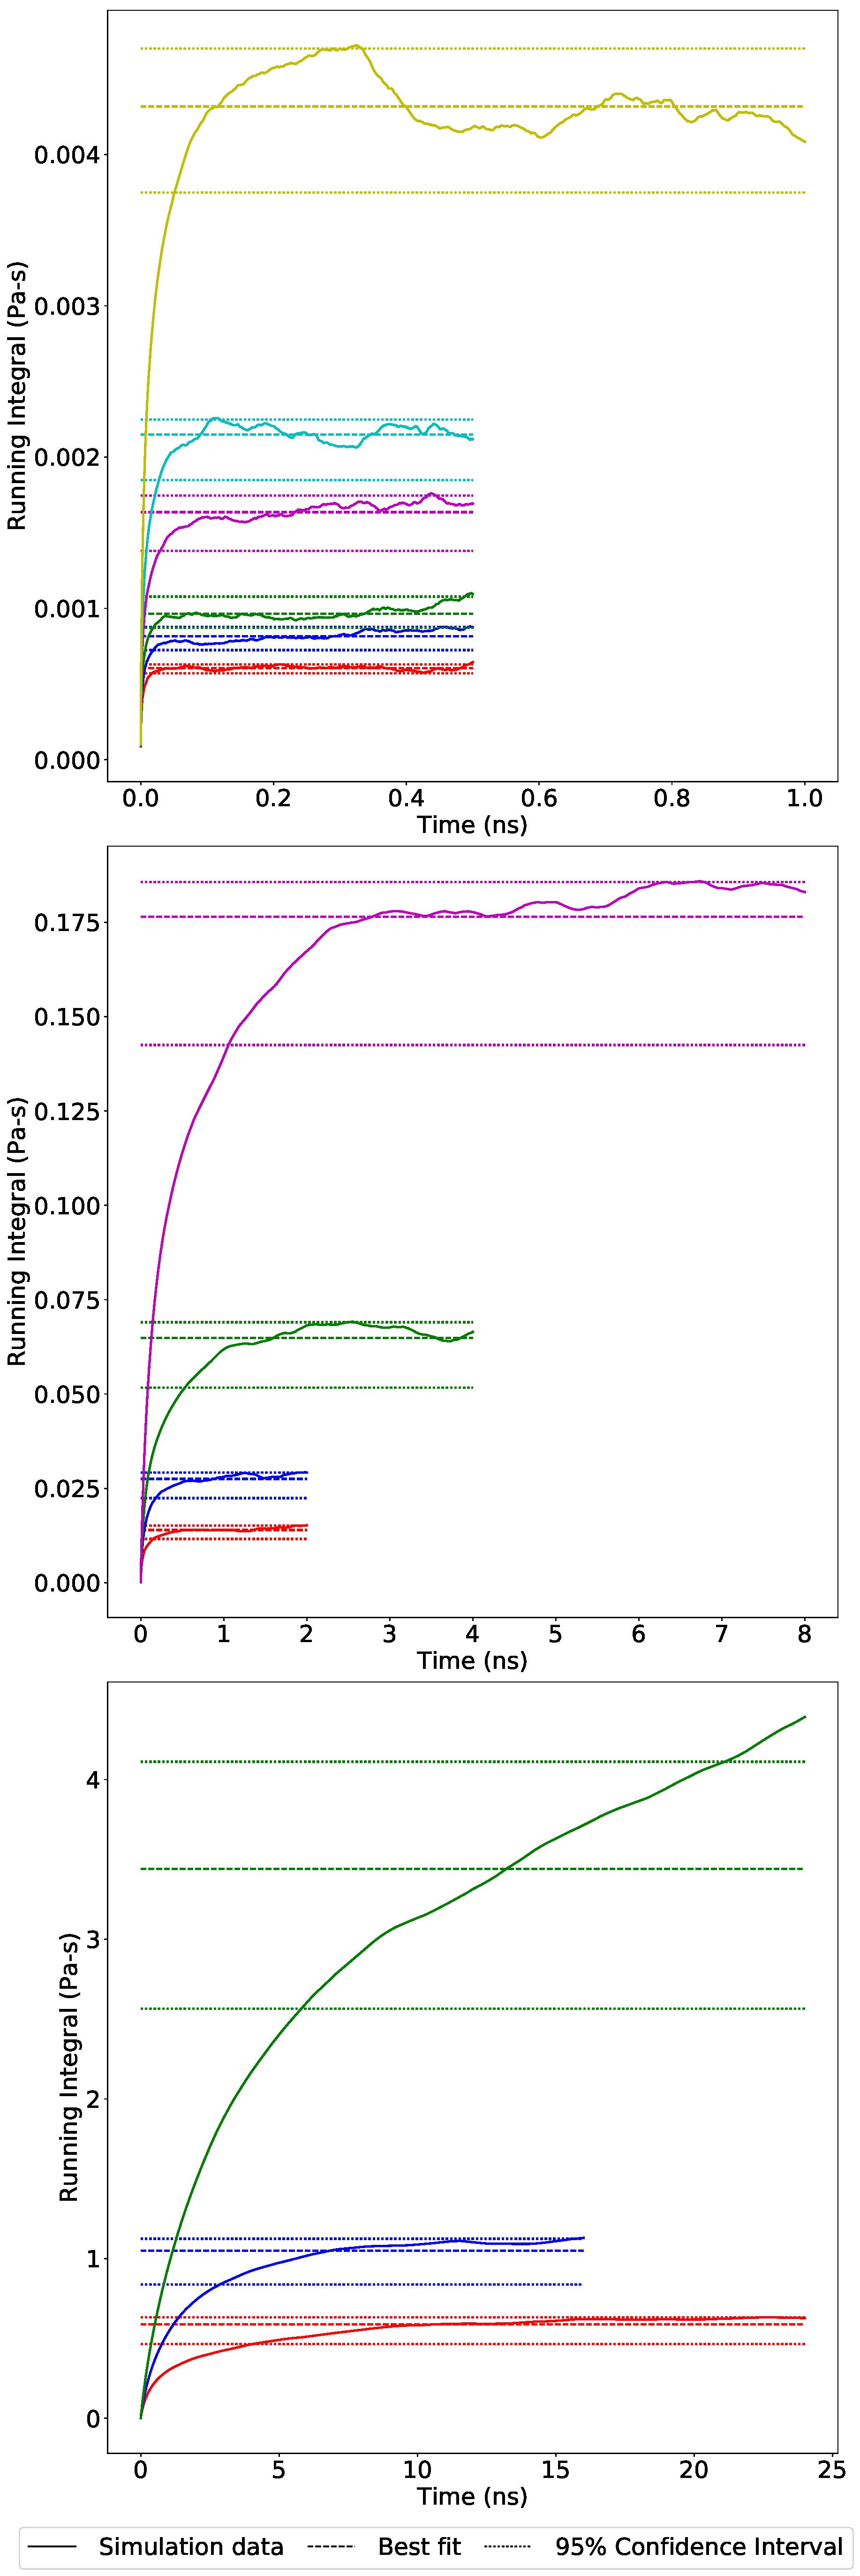
\includegraphics[width=2.6in]{GreenKubo_integrals.pdf}
		\caption{Green-Kubo integrals with respect to time. Top, middle, and bottom panels depict, respectively, low, intermediate, and high pressure/viscosity simulations where respective simulation times of 1 to 2 ns, 4 to 16 ns, and 48 to 96 ns are required to observe a Green-Kubo plateau.}
		\label{fig:running_integrals}
	\end{figure}

    \clearpage
    \newpage

    \section{Output frequency} \label{SI:Output frequency}
    
    Figure \ref{fig:compare_output_frequency} presents the average Green-Kubo integral for different output frequencies. At lower pressures ($P \le 600$ MPa) the 6 fs output frequency is required for an accurate integration. Slower system dynamics at $P \ge 700$ MPa permits similar integration accuracy for output frequencies between 12 and 36 fs.	
    
    \begin{figure}[htb!]
    	\centering
    	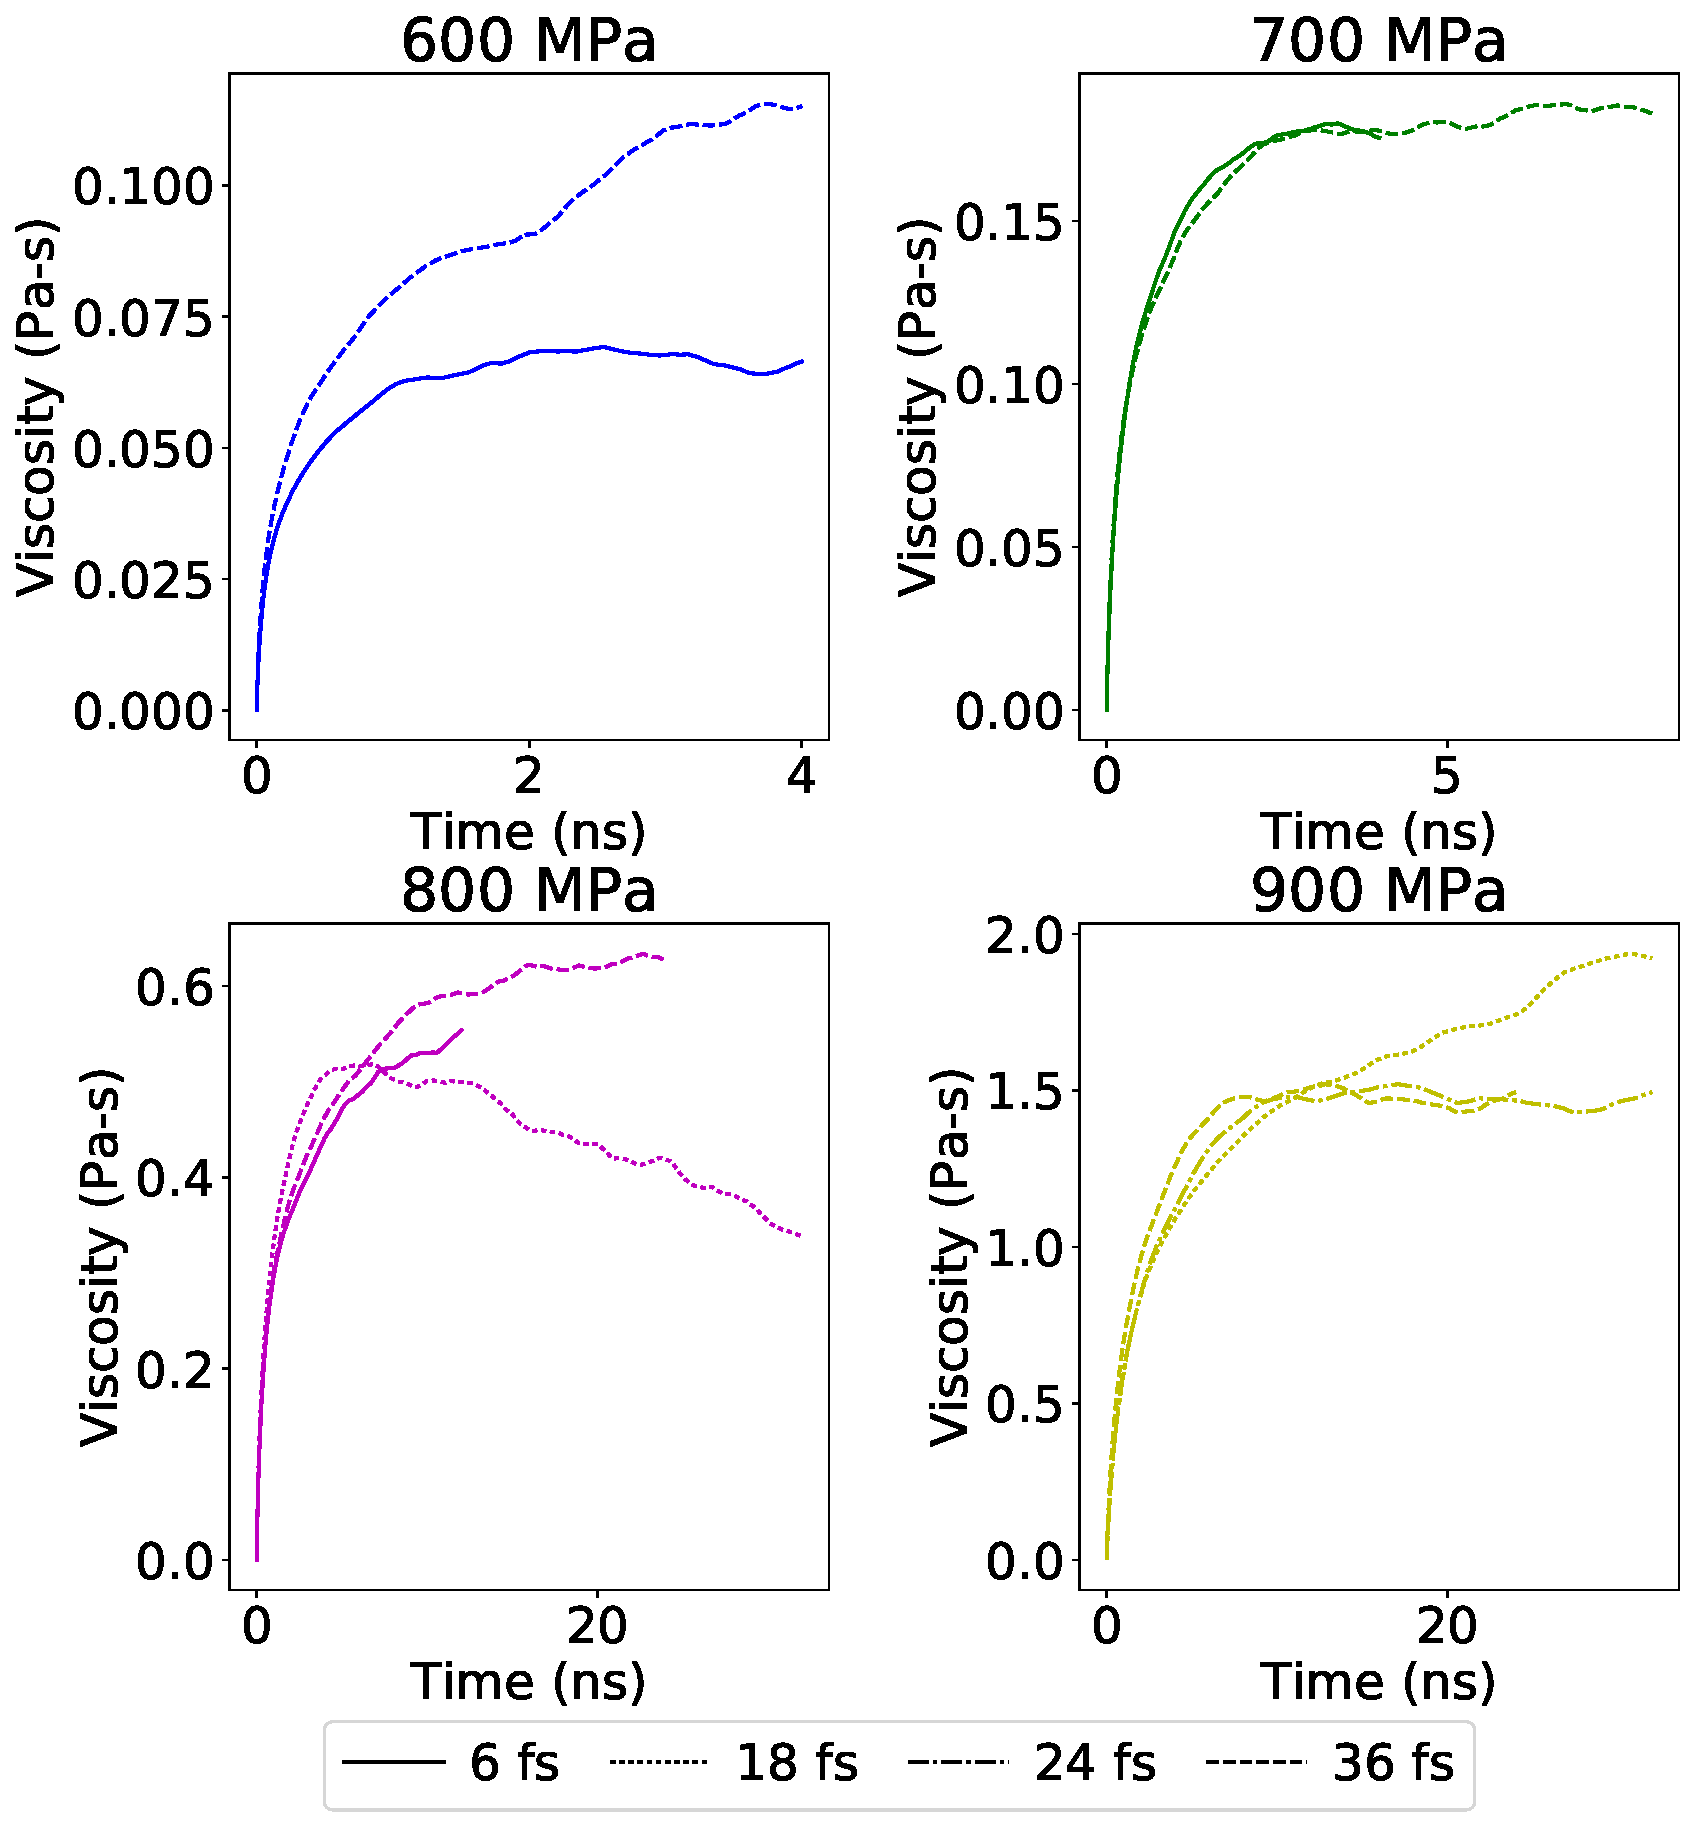
\includegraphics[width=6.4in]{output_freq_all.pdf}
    	\caption{Comparison of different output frequencies for highest pressure simulations.}
    	\label{fig:compare_output_frequency}
    \end{figure}

% depicts lower pressure/viscosity simulations where 1 to 4 ns simulations are sufficiently long. Middle panel depic Bottom panel depicts higher pressure/viscosity simulations where 8 to 48 ns simulations are required to observe a Green-Kubo plateau.
		
%	\clearpage
%	\newpage
%		
%%	\section*{References}
%	
%	\bibliographystyle{unsrt}
%	\bibliography{IFPSC_10_references}
	
\end{document}
